\documentclass[11pt]{article}
\usepackage{graphicx}
\usepackage{subcaption}
\usepackage{tabularx}
\usepackage{float}
\usepackage{listings}
\usepackage{caption}
\usepackage{amsmath}
\usepackage{algorithm}
\usepackage{algpseudocode}
\usepackage{amssymb}
\usepackage{listings}
\usepackage[inline]{enumitem}
\usepackage{xcolor}
\usepackage[top = 0.7in,bottom = 0.8in, left = 0.8in, right = 0.8in]{geometry} 

%New colors defined below
\definecolor{codegreen}{rgb}{0,0.6,0}
\definecolor{codegray}{rgb}{0.5,0.5,0.5}
\definecolor{codepurple}{rgb}{0.58,0,0.82}
\definecolor{backcolour}{rgb}{0.95,0.95,0.92}

%Code listing style named "mystyle"
\lstdefinestyle{mystyle}{
  backgroundcolor=\color{backcolour},   commentstyle=\color{codegreen},
  keywordstyle=\color{magenta},
  numberstyle=\tiny\color{codegray},
  stringstyle=\color{codepurple},
  basicstyle=\ttfamily\footnotesize,
  breakatwhitespace=false,         
  breaklines=true,                 
  captionpos=b,                    
  keepspaces=true,                 
  numbers=left,                    
  numbersep=5pt,                  
  showspaces=false,                
  showstringspaces=false,
  showtabs=false,                  
  tabsize=2
} 
\lstset{style=mystyle}

\title{\textbf{SC627 : Assignment 1}}
\author{\textbf{Adityaya Dhande}   \hspace{8mm} \textbf{210070005}}
\date{}
\begin{document}
\maketitle
\noindent
I have implemented three planners, \textbf{RRT}, \textbf{RRT*} and \textbf{PRM}. This report contains 
explanation of my implementation of these planners, followed by some 
rough hyperparameter analysis. Following this is the summary of results and 
some conclusions drawn. 
\section{Code and approach explanation}
\subsection{Common functions and structures}
\subsubsection{Graph vertex}
This struct is a template for the vertices of a graph which abstracts the different robot configurations.
It contains the angles of the robot configuration which the node represents.
\begin{lstlisting}[language=c++]
struct Node
{
    int id;
    vector<int> neighbours;
    vector<double> angles;
    Node(int nodeID) : id(nodeID) {}
};    
\end{lstlisting}
\subsubsection{Distance}
This function calculates a difference vector as the difference in angles of two configurations, wraps each element of the difference vector to a range of $[0, \pi)$
and then returns the $\ell^2$ norm of the difference vector.
\begin{lstlisting}[language=c++]
double distance(Node node1, Node node2, int numOfDOFs){
	double d = 0.0;
	for(int i = 0; i < numOfDOFs; i++){
		double diff = fmod(node2.angles[i] - node1.angles[i] + M_PI, 2 * M_PI) - M_PI;
		d += diff * diff;
	}
	return sqrt(d); 
}
\end{lstlisting}

\subsubsection{Generating random sample}
This function returns a \texttt{Node} object, containing \texttt{numOfDOFs} angles. Each of these angles are draw uniformly from 
$[0, 2\pi]$ except for the first angle, which is drawn from $[0, \pi]$ as the first link will go outside the boundary for angles greater than $\pi$.
\begin{lstlisting}[language=c++]
Node generateRandomSample(int numOfDOFs, int dummy){
    Node node(-1);
    std::random_device rd;
    std::mt19937 gen(rd());
    std::uniform_real_distribution<> dist(0, 2 * M_PI);
    for(int i = 0; i < numOfDOFs; i++){
        if( i != 0) node.angles.push_back(dist(gen));
        else node.angles.push_back(dist(gen) / 2.0);
    }
    return node; 
}    
\end{lstlisting}

\subsubsection{Checking for obstacles between two configurations}
Given two configurations $q_1$ and $q_2$, this function checks if $\bar{q} := \alpha q_1 + (1 - \alpha) q_2$
is a valid configuration where $\alpha$ is drawn using a halton sequence of 2. The values of $\alpha$
used are the first \texttt{numChecks} number of elements of $\{ \frac{1}{2}, \frac{1}{4}, \frac{3}{4}, \frac{1}{8}, \frac{5}{8}, \frac{3}{8}, \frac{7}{8}, \frac{1}{16}, \frac{9}{16}\dots \}$ 
\begin{lstlisting}[language=c++]
bool validEdge(Node node1, Node node2, int numOfDOFs, int x_size, int y_size, double *map, int numChecks){
    for (int i = 0; i < numChecks; i++) {
        double alpha = halton(i + 1, 2); 
        double interpolatedConfig[numOfDOFs];
        for (int j = 0; j < numOfDOFs; j++) 
            interpolatedConfig[j] = node1.angles[j] + alpha * (node2.angles[j] - node1.angles[j]);
        if (!IsValidArmConfiguration(interpolatedConfig, numOfDOFs, map, x_size, y_size)) 
            return false;
    }
    return true; 
}    
\end{lstlisting}

\subsubsection{K-nearest neighbours}
This function takes a list of distances and returns the indices of the K smallest entries of the list. 
It is used to find the K closest nodes from a given node.
\begin{lstlisting}[language=c++]
vector<int> KNN(const vector<double>& values, int k) {
    vector<int> indices(values.size());
    iota(indices.begin(), indices.end(), 0);
    partial_sort(indices.begin(), indices.begin() + k, indices.end(),
                        [&values](int i, int j) { return values[i] < values[j]; });
    return vector<int>(indices.begin() + 1, indices.begin() + k + 1);
}
\end{lstlisting}

\subsubsection{Breadth first search}
This function implements the breadth first search graph algorithm to find a path between two nodes. It is 
used in RRT and PRM to find the path between start and goal in the graph. 
\begin{lstlisting}[language=c++]
vector<int> findPath(const vector<Node>& nodes, int start, int goal) {
    vector<bool> visited(nodes.size(), false);
    vector<int> parent(nodes.size(), -1);
    int front = 0, rear = 1;
    vector<int> queue;
    queue.push_back(start);
    visited[start] = true;
    while (front < rear) {
        int current = queue[front];
        front++;
        for (int neighbor : nodes[current].neighbours) {
            if (!visited[neighbor]) {
                visited[neighbor] = true;
                parent[neighbor] = current;
                queue.push_back(neighbor);
                rear++;

                if (neighbor == goal) {
                    vector<int> path;
                    while (neighbor != -1) {
                        path.push_back(neighbor);
                        neighbor = parent[neighbor];
                    }
                    reverse(path.begin(), path.end());
                    return path;
                }
            }
        }
    }
    return vector<int>();
}
\end{lstlisting}

\subsection{Rapidly-exploring Random Tree (RRT)}
The \texttt{createRRT} function takes a graph (possibly empty) and adds nodes, while also forming edges, till
the graph increases to a desired size. 
\begin{algorithm}
    \caption{ : \texttt{createRRT}}\label{alg:cap}
    \begin{algorithmic}[1]
    \While{Number of nodes $<$ Desired number of nodes}
        \State  Generate a random configuration $q_{rand}$
        \State Find the node $q_{near}$ in the graph, whose configuration is closest to $q_{rand}$
        \State Calculate the angles corresponding to a potential new configuration $q_{new}$, at a distance of \texttt{STEP\_SIZE}
           from $q_{near}$, in the direction of $q_{rand}$
        \If{the path from $q_{near}$ to $q_{new}$ is obstacle free}
            \State Add $q_{new}$ to the graph and an edge between $q_{new}$, $q_{near}$
        \EndIf
    \EndWhile
    \end{algorithmic}
\end{algorithm}

In my implementation of \textbf{RRT}, first the \texttt{createRRT} function is called with the start node 
and the goal node is connected to all nodes, to which a straight obstacle free path exists, in the neighbourhood of the goal configuration. The
neighbourhood consists of K-nearest neighbours of the goal configuration in the graph. Then the BFS
graph search algorithm is used to find a path from the start node to the goal node. If no path is found, \texttt{createRRT} function is called recursively with the current 
graph to add more nodes, till a path to the goal is found.

\subsection{RRT*}
A different structure is used to store the Nodes in \textbf{RRT*}, which stores the parent
of each node and also the cost of each node. The cost of a node is defined as 
$$\texttt{cost}(q) = \texttt{cost}(\texttt{parent}(q)) + \texttt{distance}(q, \texttt{parent}(q))$$
\begin{lstlisting}[language=c++]
struct StarNode
{
    int id, parent;
    double cost;
    vector<double> angles;
    StarNode(int nodeID) : id(nodeID) {}
};
\end{lstlisting}
\textbf{RRT*} is similar to \textbf{RRT} with a few changes in how the graph is formed. 
The way the path is found in \textbf{RRT*} is different in my implementation. The path is formed in reverse, 
by starting from the goal node and moving to the parent node recursively till the start node is reached.

For the graph formation, a potential new node is calculated in the same way as in \textbf{RRT}. Instead 
of connecting this to the closest node in the graph, it is connected to the node with the least cost in its neighbourhood (if the straight line path between the two nodes is obstacle free).
The neighbourhood is decided by a fixed radius in my implementation. After the edge is formed with a node in the neighbourhood, I check the remaining nodes in the neighbourhood
and see if forming an edge with the new node reduces the cost of those nodes, and change the parent of those nodes accordingly. 

\subsection{Probabilistic Road Map (PRM)}

The \texttt{createPRM} function takes a graph (possibly empty) and adds nodes, while also forming edges, till
the graph increases to a desired size. 
\begin{algorithm}
    \caption{ : \texttt{createPRM}}\label{alg:cap}
    \begin{algorithmic}[1]
    \While{Number of nodes $<$ Desired number of nodes}
        \State  Generate a random configuration $q_{rand}$
        \State Add $q_{rand}$ to the graph if it is a valid configuration.
    \EndWhile
    \For{\texttt{node1} in \texttt{graph}}
        \For{\texttt{node2} in \texttt{neighbourhood(node1)}}
            \If {the straight path between \texttt{node1} and \texttt{node2} is obstacle free}
                \State Add an edge between \texttt{node1} and \texttt{node2}
            \EndIf 
        \EndFor
    \EndFor
    \end{algorithmic}
\end{algorithm}

In my implementation of \textbf{PRM}, first a graph of a fixed size is formed, using \texttt{createPRM}, and the start and goal nodes are connected to this
graph in a similar way as done with the goal node in \textbf{RRT}. Then BFS graph algorithm is used
to find a path between the start and goal nodes. If a path is found then it is returned, and if no path is found, \texttt{createPRM} is called with the current graph to 
increase its size by adding more nodes and this process is repeated recursively till a path is found between the start and goal nodes. 

\subsection{Effect of Hyperparameters}
The following are the hyperparameters encountered in the planners :
\begin{itemize}
    \item \textbf{Incremental number of nodes} : From observation, increasing the nodes by $n$ and then again by $n$ takes more compute time than increasing nodes by $2n$ in one go, so a low value is not preferred. A high value also causes some unecessary computation when only a few additional nodes would suffice. A low value could also cause the cost to be high if a path is found.
    \item \textbf{Initial number of nodes} : A very high value increases time requirement for a lot of start and goal configurations. A low value will need more increments and causes increase in computation. A low value could also cause the cost to be high if a path is found.
    \item \textbf{Number of neighbours in neighbourhood} :  A low value could cause the cost to be high if a path is found. Low value decreases chances of finding a path. High value increases computation.
    \item\textbf{ STEP$\_$SIZE in RRT and RRT*} : Small step size causes a denser tree formation which increases the computation where as large step size will not give a fine path and the path will have high cost. 
    \item \textbf{Neighbourhood radius in RRT*} : Large neighbourhood radius increases computation and a small neighbourhood radius increases the cost of the path.
    \item \textbf{Number of points to check for obstacle free path} : From observation, this has not significantly affected planning time.
\end{itemize} 

\section{Results}

\begin{table}[H]
    \begin{center}
        \caption*{Comparision of different planners}
        \vspace{-2mm}
        \begin{tabular}{|c|c|c|c|}
            \hline
             Field &  \textbf{RRT} & \textbf{RRT*} & \textbf{PRM} \\
            \hline
            Average planning time  &  2.337s & 2.976s   &  \textbf{2.096s} \\
            \hline
            Success rate for $<$ 5s   &  $100 \%$ & $100 \%$ &  $95 \%$\\
            \hline   
            Average path cost   &  4.263 & \textbf{3.043 }  &  3.838\\
            \hline     		
            Average number of nodes   &  1000 & 1000   &  1030\\
            \hline     	
            Max planning time  &  \textbf{3.039s} & 3.695s   &  5.222s \\
            \hline
            Max path cost   &  15.056 & \textbf{7.639 }  &  10.099\\
            \hline     		
            Max number of nodes   &  1000 & 1000   &  1600\\
            \hline     		
        \end{tabular}
    \end{center}
 \end{table}
\vspace*{-7mm}
 \begin{figure}[H]
    \centering
    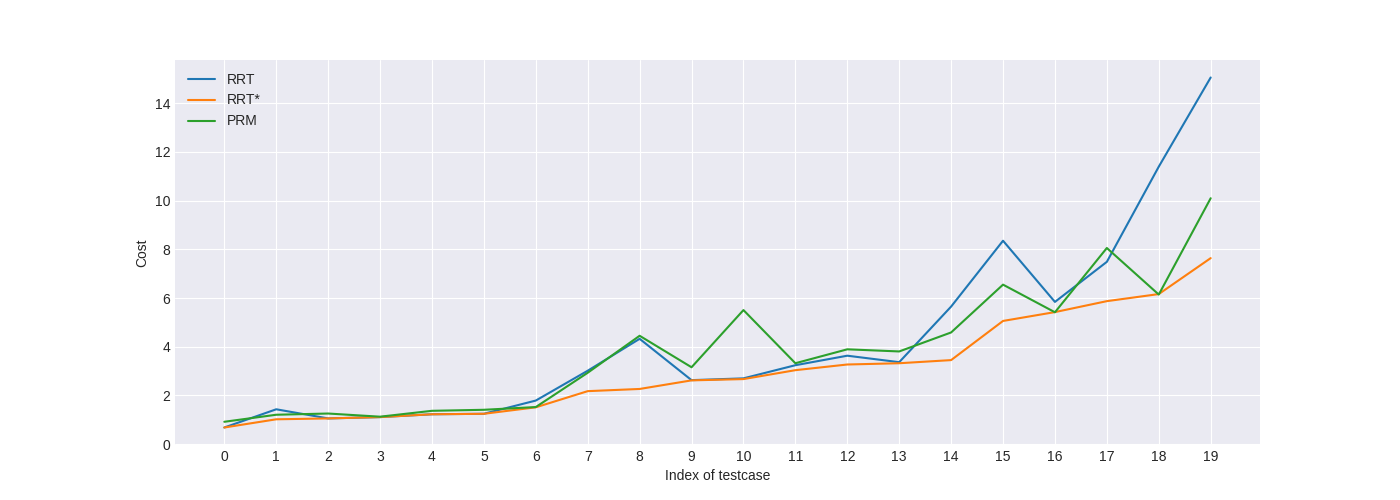
\includegraphics[width=\linewidth]{plot1_1000.png}
    \caption*{Costs of different planners}
\end{figure}

\begin{figure}[H]
    \centering
    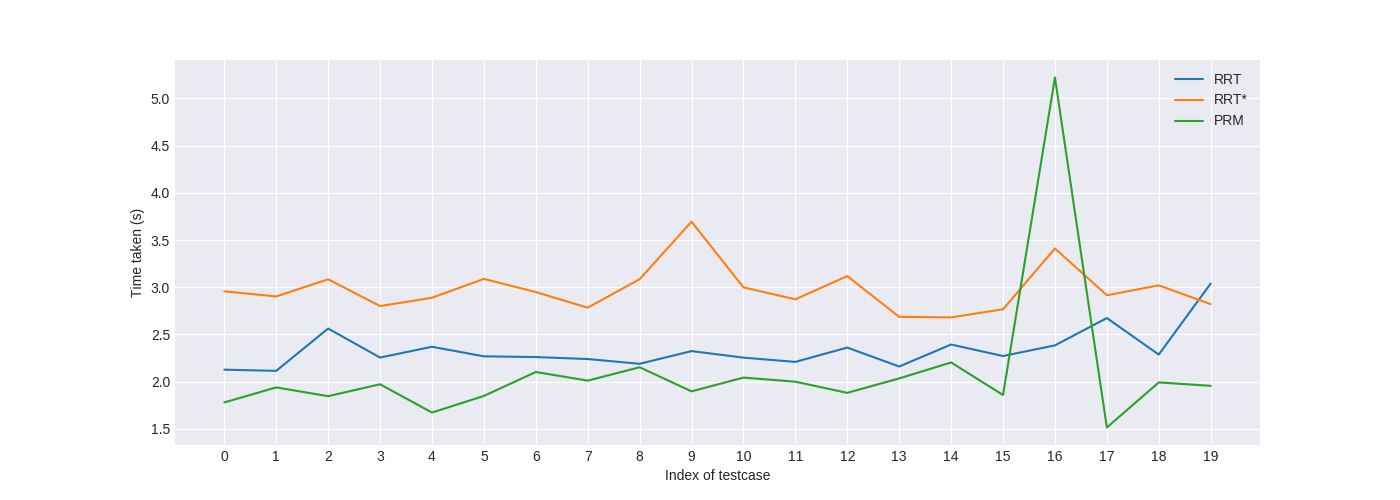
\includegraphics[width=\linewidth]{plot2_1000.png}
    \caption*{Time taken by different planners}
\end{figure}
\vspace*{-8mm}
\begin{figure}[H]
    \centering
    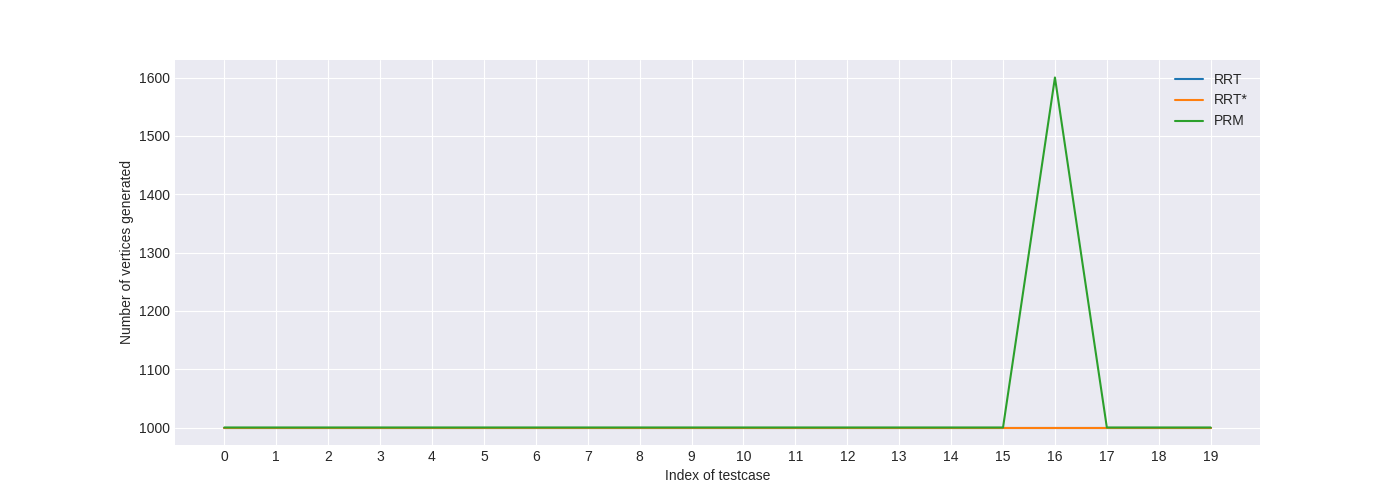
\includegraphics[width=\linewidth]{plot3_1000.png}
    \caption*{Number of nodes generated by different planners}
\end{figure}
\subsection{Summary and explanation of results}
The \textbf{number of nodes} is the same for all the planners except for one test case where \textbf{PRM}
generates a larger number of nodes. The variance in number of nodes for all the planners was more
when I used different hyperparameters. For lower \textbf{initial number of nodes} and lower \textbf{incremental number of nodes}
some testcases had lower than 1000 nodes generated but the time taken for many testcases exceeded 5 seconds. 

\noindent
\textbf{PRM} takes lesser \textbf{time} on average compared to \textbf{RRT} and \textbf{RRT*} because it is computationally cheaper. 
This is because for a given \textbf{number of initial nodes}, \textbf{PRM} first samples the nodes and then forms the edges. Where as in the other methods
the edges are formed and only if a valid edge is found the sample is added to the graph. \textbf{RRT} still is faster than \textbf{RRT*} as after forming a 
node in a similar fashion to \textbf{RRT}, \textbf{RRT*} finds nodes in a \textbf{neighbourhood} and forms new edges that minimise the cost of all the edges in the neighbourhood. 

\noindent
The consistent trend in \textbf{cost} is that \textbf{RRT*} performs better than \textbf{RRT} and \textbf{PRM}.
This is expected because whenever a new node is added, it forms an edge only with the node in its neighbourhood which will give it the lowest cost from the start node. \textbf{RRT} and \textbf{PRM} form edges with the closest nodes. Using a cost in \textbf{PRM} might perform as good as \textbf{RRT*} with the use of a weighted graph search algorithm like \textbf{Dijkstra's algorithm}.
\subsection{Best planner for the environment}
\begin{itemize}
    
    \item I think \textbf{RRT*} planner is the most suitable for the environment as even though it takes more time than \textbf{RRT} and \textbf{PRM} it is consistent and the time taken is still reasonable. \textbf{PRM} has a high variance in the time taken and goes to high values some times. \textbf{RRT*} also generates fewer or same number of nodes as \textbf{RRT} and \textbf{PRM} and the most cost effective path amongst the three planners.
    \item The issues with my implementation of \textbf{RRT*} are on quite a few testcases it gave a path with the almost the same cost as \textbf{RRT} and \textbf{PRM} while taking relatively more time.  
    \item Additional hyperparameter tuning will improve both the time and cost performance of my implementation of the \textbf{RRT*} planner. The \textbf{neighbourhood radius} and \textbf{STEP\_SIZE} significantly affect the time and cost performance of the planner. They can be tuned for a specific environment to improve the performance of the planner. 
\end{itemize}
\newpage
\section{Compiling the code}
\begin{lstlisting}[language=bash]
    g++ planner.cpp -o planner.out      # Compiles the planner.cpp
    g++ -O3 planner.cpp -o planner.out  # Compiles planner.cpp using optimised compiler\end{lstlisting}
    
    These commands can be used to compile the code. 
\end{document}